\section{Motivation}

\todo{Add abbreviations page!}

Each year, the robotic community gathers at conferences such as IROS
(International Conference on Intelligent Robots and Systems), where they
exhibit their discoveries and achievements in the field. For the year 2019, the
Drone Racing League will be hosting a series of races in which autonomous drones
will compete and attempt to outperform a professional FPV (First Person View)
drone pilot.\\

\begin{figure}[h]
	\centering
	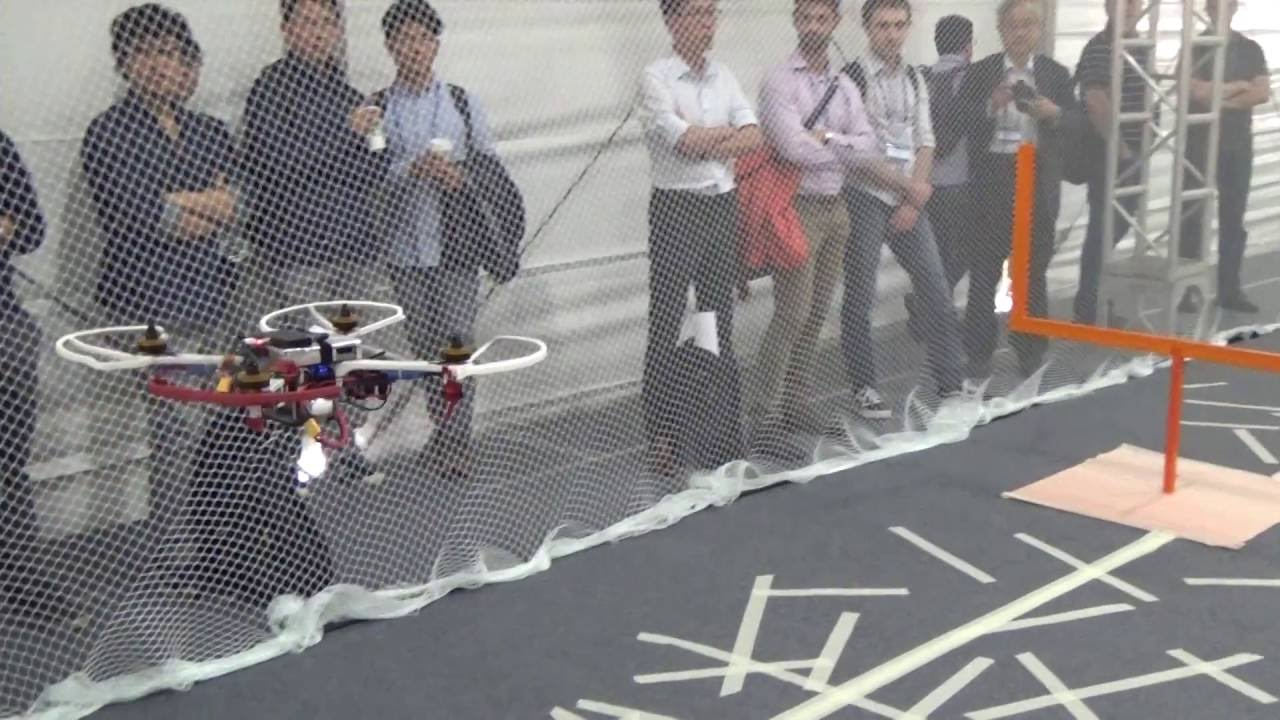
\includegraphics[width=0.5\textwidth]{figure/iros_2016.jpg}
	\caption{Autonomous drone racing "arena" at IROS 2016.}
	\label{fig:iros}
\end{figure}

The company \emph{Lockheed Martin} is sponsoring the event and offering a prize of 2
million USD for the winning team~\cite{LockheedDRL}. Teams of university
students and other drone enthusiasts shall present innovative approaches on
vision-based systems for unmanned aerial vehicles: hence, they showcase their
progress through racing.\\

\subsubsection{Beyond the hype and into reality}
The rise of consumer drones during the recent years indicates a craze for UAVs
(Unmanned Aerial Vehicle) from the average citizen. First seen as nothing more
but toys, the now well-known quadcopters are revealing their full potential,
thanks to the breakthroughs of robotics engineers and large businesses combining
their expertise to offer futuristic services.

Be it Amazon's yet to come \emph{Prime Air} service~\cite{PrimeAir}, promising
30 minutes deliveries by autonomous drones in a short radius of their
facilities, or even Ehang's electric sky-taxis driving a human passenger for up
to 10 miles~\cite{Ehang184}, more and more innovative companies are
demonstrating the possible applications of those agile fliers.  Indeed, it seems
this fantastic future is not far from our reach. \emph{Amazon Prime Air}
successfully delivered a package to its first customer in December
2016~\cite{PrimeAirFirst}, which took only 13 minutes and did not involve a
human pilot.\\

Moreover, reports from \emph{Goldman Sachs} \cite{TopTal} estimated that the
drone market would reach 100 billion USD between 2016 and 2020, referring to the
military, consumer and commercial sectors.%, as shown on
%Figure~\ref{fig:toptal}.\\

%\begin{figure}[h]
	%\centering
	%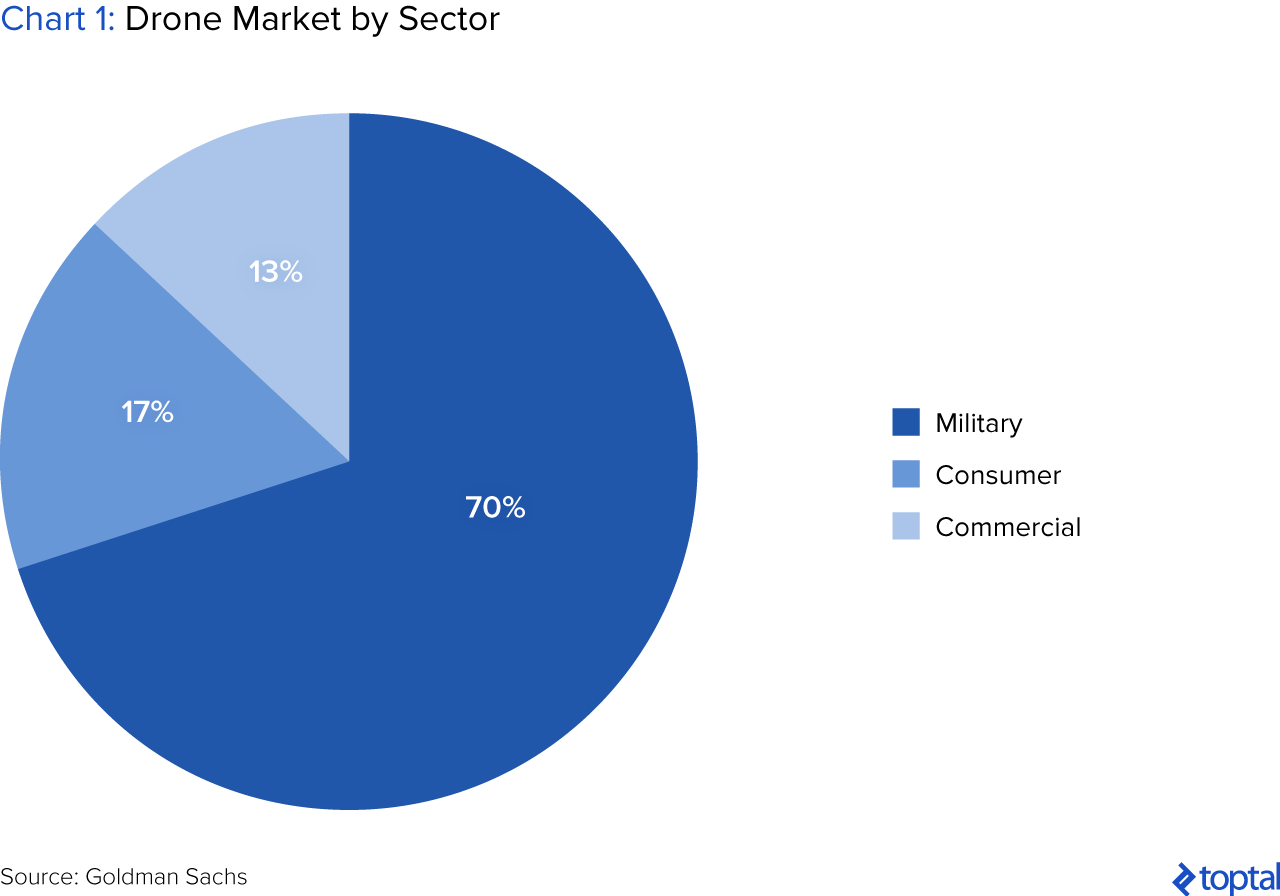
\includegraphics[width=0.7\textwidth]{figure/toptal.png}
	%\caption{Drone market by sector: estimates for 2016-2020~\cite{TopTal}.}
	%\label{fig:toptal}
%\end{figure}

Based on those figures, it is safe to assume that autonomous drones hold a
promising future, and that active research in the field will not go to waste.
After all, autonomous drone racing might be a recreational segue to faster and
more precise self-flying vehicles for all industries.
